\section{Koordinater generelt}
I matematikafsnittet med polære koordinater, \cref{mat:sec:trig}, blev et relevant eksempel på et anderledes koordinatsystem end de kartesiske koordinater ($x,y,z$ koordinater) gennemgået, som kan være en fordel at benytte til at beskrive sit system. Indenfor mekanik er det netop denne tilgang, man har til koordinatsystemer. Man benytter dem som et redskab, til at beskrive sit system bedst og lettest muligt. Der er ikke en dybere fortolkning af ens valg af koordinater.

For eksempel kan et to-dimensionelt system beskrives med to rumlige, kartesiske, koordinater, $x$ og $y$. Man velkommen og indenfor al ret til at beskrive systemet med flere en de to koordinater, som så vil afhænge af hinanden. Kompleksiteten af et problem mindskes oftest ved at begrænse mængden af koordinater anvendt til den mindst nødvendige mængde. Ethvert almindeligt klassisk problem kan altid beskrives ud fra tre rumlige dimensioner per objekt/legeme i systemet.

Generelt er et valgt koordinatsystem udtryk for, hvor mange dimensioner det forventes, at der skal bruges for nøjagtigt at beskrive problemet. Dette hænger sammen med, hvor mange retninger et legeme kan bevæge sig i uafhængigt af andre retninger. Eksempelvis kan to uafhængige variable $a$ og $b$, samt en variabel $f(a,b)$ betragtes. At $a$ og $b$ er uafhængige af hinanden betyder, at hvis værdien af $a$ ændres, så ændres værdien af $b$ ikke, og omvendt. Modsat er $f(a,b)$ afhængig af både $a$ og $b$, og kan derved ikke kaldes en uafhængig variabel. Ofte støder man på variable, der er implicit afhængige, hvilket betyder at man ikke skriver (eksplicit) at variablen afhænger af en anden. I \cref{mat:sec:trig} så vi et eksempel på dette. Forsøger man at beskrive kuglen på snoren med kartesiske koordinater ($x$ og $y$), så er begge nødvendige, da kuglens bane krummer. Banen kunne dog beskrives med vinklen i polære koordinater. Begrænsningen på systemet, at kuglen kun kan bevæge sig på cirklen, gør de kartesiske koordinater skal opfylde Pythagos' sætning: $x^2 + y^2 = l^2$, hvor $l$ er snores længde. De kartesiske koordinater er derfor afhængige, som kommer af en fysisk begrænsning på systemet. Man siger derfor at $x$ og $y$ er implicit afhængige.
% Dette ses tit med koordinater, hvor man ofte skriver eksempelvis $x$ i stedet for $x(t)$, idet man antager det for kendt, at $x$ afhænger af $t$. Dette er vigtigt, da man ønsker at beskrive systemet med så få uafhængige koordinater som muligt. % Dette er uklart i forhold til tidsafhængighed og frie variable. Der skelnes ikke her mellem frie variable som t, og de variable vi finder udtryk for til at beskrive vores system (som afhænger af enten t eller en anden tidsafhængig variabel).
%

% At koordinatsystemet her betragtes som givende udtryk for det forventede antal uafhængige bevægelser, forklares ud fra, at det ikke altid kan vides på forhånd, hvorvidt en variabel er afhængig af andre variable eller ej. Dette finder man ud af, når man analyserer systemet, som man har med at gøre, hvorefter man kan tilrette sine koordinater efter det. Som eksempel på dette tages et simpelt pendul, som vi vil analysere senere. Umiddelbart kan pendulets bevægelse beskrives ud fra to kartesiske koordinater, $x$ og $y$, der varierer i tiden $t$, eller alternativt med to polære koordinater, med en vinkel $\phi$ og en pendullængde $r$, der også begge varierer med tiden. I dette tilfælde viser det sig dog, at længden $r$ er konstant og ikke variabel, hvormed systemet burde kunne beskrives udelukkende ud fra et udtryk for vinklen $\phi$ til tiden $t$. Men hvad med de to kartesiske koordinater $x$ og $y$? Her kan det senere vises, at den ene af de to koordinater er overflødige, da der kan findes et funktionsudtryk, som beskriver pendulets bevægelse i den ene retning ud fra dens bevægelse i den anden. Dette er dog ikke altid tilfældet, hvormed det giver god mening, at starte ud med begge koordinater. Herefter kan man altid fjerne koordinater, der ikke er nødvendige, ved ændre på sit koordinatsystem. \\

Som det vil blive nævnt senere i afsnittet om generaliserede koordinater, så er det smart at vælge sine koordinater, efter at man har gjort sig nogle indledende overvejelser omkring sit system, for at begrænse den kompleksitet af ens beskrivelse af et system. Tit vil ens system nemlig have symmetrier eller lignende restriktioner i sin bevægelse, som så vil sætte begrænsninger på antallet af koordinater (senere nævnt som frihedsgrader), der er nødvendige for at beskrive systemet. Dette bliver anvendt til, at løse de fleste af systemer I bliver præsenteret for på campen.% Udover at nævne pendulet som eksempel igen, er det dog værd at nævne, at mange systemer, med to legemer, har disse begrænsninger, og flere endda kan reduceres til kun at have en variabel (i stedet for to til hvert legeme), hvormed hele systemets bevægelse kan beskrives ved bare at kende en enkelt værdi.

\begin{figure}[]
    \centering
    \begin{tikzpicture}[line width=2pt]
        \coordinate (o) at (0,0);
        %
        \draw[-{Stealth[length=5mm, width=3mm]}] (o) to (4,0);
        \draw[-{Stealth[length=5mm, width=3mm]}] (o) to (0,4);
        \draw[-{Stealth[length=5mm, width=3mm]}] (o) to ++(-131:3.6cm);
        %
        \draw (-126.5:3.3cm) node[anchor=south west]{\LARGE $x$};
        \draw (3.9,-0.09) node[anchor=north east]{\LARGE $y$};
        \draw (0.09,3.9) node[anchor=north west]{\LARGE $z$};
        %
        \draw[dashed, line width=1pt] (o) to ++(-45:2.5cm) to ++(90:4cm);
        \draw[-{Stealth[length=4mm, width=2.5mm]}] (o) to ++($ (-45:2.5cm) + (90:4cm) $);
        \draw [domain=-129:-45, line width=1.5pt] plot ({0.65*cos(\x)}, {0.65*sin(\x)});
        %
        \draw (-87:6.5mm) node[anchor=north]{\LARGE $\phi$};
        \draw (-47.5:1.25cm) node[anchor=south west]{\LARGE $r$};
        \draw ($ (-45:2.5cm) + (90:2.5cm) $) node[anchor=west]{\LARGE $z$};
        \draw ($ (-45:1.4cm) + (90:2.15cm) $) node[anchor=south east]{\LARGE $\va{r}$};
    \end{tikzpicture}
    %
    % 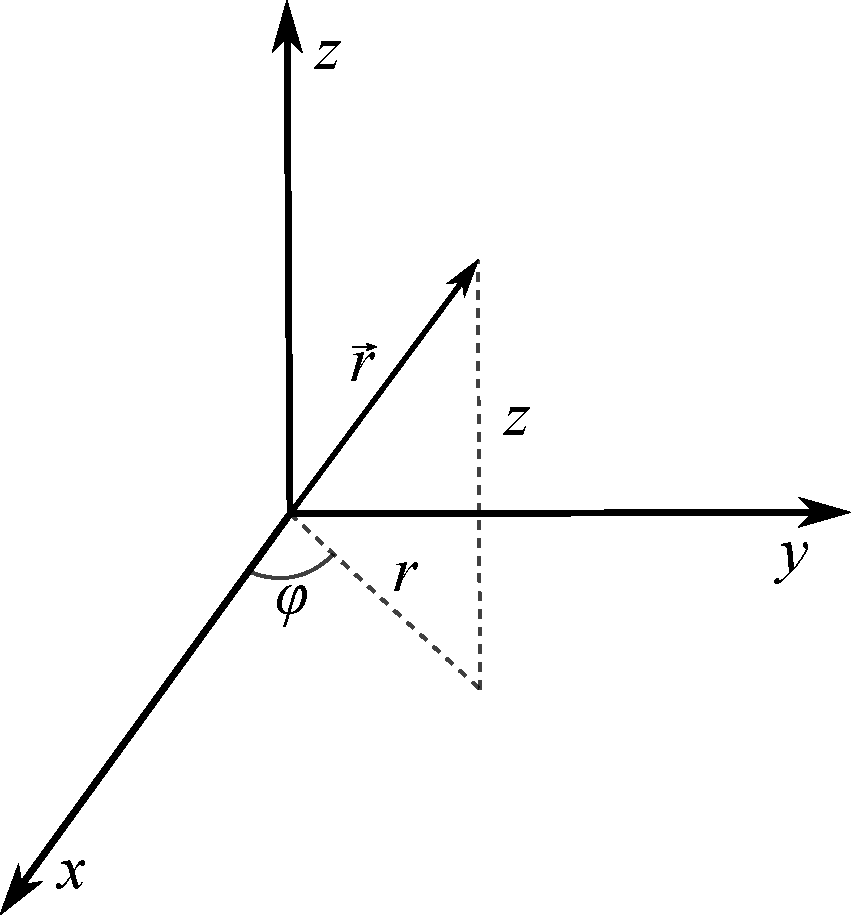
\includegraphics[width=.4\textwidth]{Mekanik/figurer/CylindriskeKoordinater.pdf}
    \caption{Det cylindrisk polære koordinatsystem er en tredimensionel udvidelse af det todimensionelle polære koordinatsystem fra \cref{mat:sec:trig}. Her defineres en plan med en polærakse, der udspændes af et polært koordinatsystem med koordinaterne $r$ og $\phi$. Polærplanen kan så forskydes langs en akse gennem origo vikelret på planen, og denne forskydning er det tredje koordinat kaldet $z$. Det polære $z$-koordinat er det samme som det kartesiske $z$-koordinat, mens $r$ og $\phi$ fungerer som i det todimensionelle, polære koordinatsystem.}
    \label{fig:CylindriskeKoordinater}
\end{figure}
%
\subsubsection{Cylindrisk polære koordinater}
Til beskrivelsen af legemer, der bevæger sig i kurvede baner, benyttes ofte cylindriske koordinater i stedet for kartesiske koordinater. Cylindriske koordinater er en tredimensionel udvidelse af de todimensionelle polære koordinater. Det 3. koordinatet, $z$, forskyder planen, de polære koordinater $r,\phi$ udspænder, langs aksen, der er ortogonal (vinkelret) på planen. I polære koordinater defineres et punkt som origo, det vil sige $(0,0,0)$, og ud fra det en polærakse, der angiver placeringen af vinklen på $\phi = 0$. Et punkts afstand til origo, $r$, og dets vinkel med polæraksen, $\phi$, angiver så de polære koordinater. Defineres koordinatsystemet således at polæraksen og $x$-aksen i et tilsvarende kartesisk koordinatsystem er sammenfaldende, ville $\phi$ være vinklen ift. $x$-aksen i $xy$-planen og $z$ er forskydningen ift. polærplanen, se \cref{fig:CylindriskeKoordinater}. Det bemærkes, at det kartesiske 3. koordinat og det cylindriske 3. koordinat er ens, og at afstanden $r$ ved udvidelsen fra polære til cylindriske koordinater forbliver uændret; det vil sige at en ændring i $z$ ikke giver en ændring i $r$. Da der kun fokuseres på legemers rotation om én akse, kan $z$-aksen defineres til at være denne rotationsakse, hvorved det cylindriske 3. koordinat forbliver uændret i tid.  \\

I polære koordinater er der en meget nyttig sammenhæng mellem et legemes totale fart og den tidsafledte af vinkelkoordinatet $\dv*{\phi}{t}$. Det antages at førstekoordinatet, $r$, er konstant i tid, $\dv*{r}{t} = 0$. Derfor kan \cref{mat:eq:kartesisk/polaer} fra matematikafsnittet\footnote{I matematikafsnittet hedder vinklen $\theta$, hvor den her hedder $\phi$. Det betyder ikke det store hvad man kalder den, men for pendulet er det almindelig at bruge $\phi$, hvorfor det også gøres her i kapitlet.} benyttes til at opskrive de tidsafledede af de kartesiske koordinater udtrykt ved de polære koordinater
%
\begin{align}
\begin{aligned}
	\dot{x} &= -r\sin(\phi)\dot{\phi} \: , \\
	\dot{y} &= r\cos(\phi)\dot{\phi} \: .
\end{aligned}
\end{align}
%
Da hastighed er en vektor, $\vb{v} = \dot{x} \vu{x} + \dot{y} \vu{y}$, så er den totale fart længden af hastighedsvektoren, og den kan bestemmes vha. Pythagoras sætning, \cref{pythagoras2.5},
%
\begin{align} \label{mek:eq:SmartFart}
\begin{aligned}
	v &= \sqrt{\dot{x}^2 + \dot{y}^2} = \sqrt{(-r\sin(\phi)\dot{\phi})^2 + (r\cos(\phi)\dot{\phi})^2} = \sqrt{r^2\dot{\phi}^2 \left(\cos^2(\phi) + \sin^2(\phi) \right)} \\
	&= r\dot{\phi}\sqrt{\cos^2(\phi) + \sin^2(\phi)} = r\dot{\phi}.
\end{aligned}
\end{align}
%
Her er grundrelationen $\cos^2(\phi) + \sin^2(\phi) = 1$ benyttet, og dette resultat bliver meget anvendeligt, når der skal bestemmes energier for roterende legemer. Det er en essentiel del af Lagrangemekanikken, som kommer senere. Differentieres \cref{mek:eq:SmartFart} igen med hensyn til tid fås
%
\begin{align} \label{mek:eq:vinkelacceleration}
	a = r\ddot{\phi}.
\end{align}

For at illustrere hvordan disse betragtninger om koordinatsystemer kan bruges i en virkelig situation, men også hvordan Newtonsk mekanik let kan komme på dybt vand og blive kluntet at håndtere, kigges nu på et pendul.